\pdfoutput=1

\documentclass{l4proj}

%
% put any packages here
%

\newcommand{\code}[1]{\texttt{#1}}

\begin{document}
\title{Who To Follow In Context}
\author{Darren Burns}
\date{\today}
\maketitle

\begin{abstract}
TODO ABSTRACT GOES HERE
\end{abstract}

\educationalconsent
%
%NOTE: if you include the educationalconsent (above) and your project is graded an A then
%      it may be entered in the CS Hall of Fame
%
\tableofcontents
%==============================================================================

\chapter{Introduction}
\pagenumbering{arabic}
The first page, abstract and table of contents are numbered using Roman numerals. From now on pages are numbered
using Arabic numerals. Therefore, immediately after the first call to $\backslash$chapter we need the call
$\backslash$pagenumbering$\{$arabic$\}$ and this should be called once only in the document. 

The first Chapter should then be on page 1. You are allowed 50 pages for a 30 credit project and 35 pages for a 
20 credit report. This includes everything up to but excluding the appendices and bibliograph, i.e. this is a limit on
the body of the report.

You are not allowed to alter text size (it is currently 11pt) neither are you allowed to alter the margins.

Note that in this example, and some of the others, you need to execute the following commands the first time you process the files.
Multiple calls to pdflatex are required to resolve references to labels and citations. The file bib.bib is the bibliography file.

\begin{verbatim}

            > pdflatex example0
            > bibtex example0
            > pdflatex example0
            > pdflatex example0

\end{verbatim}


\section{Goal}
The aim of this project was to create an application which provides a relevant set of Twitter accounts to follow based on an input query. In particular, we are interested in recommending accounts which are relevant at the current moment in time. Therefore, a large portion of the project is concerned with providing real-time updates and corrections to recommendations based on the evidence provided via a stream of Twitter statuses.


\section{Motivation}
Recommendations are becoming an increasingly important aspect of digital systems. Celma \& Lamere (ISMIR 2007) noted that 2/3 of movies rented via Netflix were through recommendation, and 35\% of sales made via Amazon are through recommendation. Although numerous factors can influence these figures (such as the ratio of the area of the UI displaying recommendations to the area displaying standard site content), they undoubtedly show that recommender systems greatly improve user retention and interaction.

From a social media perspective, recommending interesting people to follow is exceptionally important in retaining users. When a user initially signs up for a service such as Twitter, they will not see any tweets unless they follow users. Through quality recommendations, the user is more likely to see content that they are interested in and thus they are more likely to continue to use the site. For social media platforms which heavily rely on advertising revenue for income, keeping users engaged and looking at their news feeds is of particular importance.

\section{Related Works}

\subsection{Twitter Search}
Twitter’s existing search service allows searching for accounts based on a search query. This is very similar to the purpose of this project. However, this project displays and updates results in real-time, and new evidence is applied immediately. Therefore if a result page is left open, then the ranking of accounts will be adjusted as people start and stop discussing the query topic. This project intends to provide a live window into ongoing events, and the real-time nature of the displayed results reflects this.

\subsection{Who To Follow at Twitter}
“WTF” was the service used at Twitter which recommended accounts to follow based on the people already followed by an account. The primary difference between this project and Twitter’s initial Who To Follow system is that this project relies on information retrieval and learning to rank methods which rely entirely on the content of the tweets that users write, whilst Twitter relied on graph analysis, which examines interactions between users to try and identify users similar to those the author already follows. Since the initial deployment of this service in 2010, Twitter announced they are reimplementing the service using Pig and Hadoop to improve scalability, and also to apply machine learning approaches using a wider variety of signals.

\subsection{Klout}
Klout provides a well-known system for ranking the influence of users across numerous social media platforms and online communities. It takes into account over 3600 features from these sources, and processes around 500 million user interactions each day.


\chapter{Requirements}
Requirements

\chapter{User Interface}
User interface

\chapter{System Architecture}

    \section{Server Architecture}

On the server side the architecture consists of multiple different components each with their own distinct responsibilities. These components are described in the following subsections.

        \subsection{The Actor Model}
The real-time nature of the application means that if performance is poor then it will immediately impact user experience. Should feature extraction for a user timeline take longer than expected, then a user will have to wait until the system gets around to processing that user. As such, high levels of concurrency were deemed vital in order to meet user requests in a timely manner. To accommodate such a requirement, the system was designed using the \textit{Actor model}.

Actor systems provide an alternative means of concurrency that avoid the pitfalls of typical synchronisation methods such as the use of shared state with locking. The actor model of concurrency was first popularised by the Erlang programming language, and has increased in popularity in recent years with the release of applications such as WhatsApp which use the model extensively. An actor system consists of a set of actors. Actors are entities capable of performing some computation on a thread in response to messages. Actors also have the ability to create new “child” actors, and to send messages to other actors in the system, who will then react in their own way depending on the information contained within that message. By communicating between actors solely through asynchronous \textit{immutable} message passing, we guarantee that the computations performed by a single actor cannot result in issues such as thread interference.

        \subsection{Reactive Systems}
        The architecture of the system is implemented to conform to many of the tenets described in the ``Reactive Manifesto''. That is, the system architecture is designed to be responsive, resilient, elastic, and message-driven.
        
            \subsubsection{Responsiveness}
            Responsiveness is a key aim of the application. Messages passed from actor to actor in potential bottlenecks are load-balanced in order to minimise the work queued on a single actor or thread and maximise throughput. Within each defined actor is a response time guarantee which, if not met, causes the actor to be restarted in attempt to regain responsiveness. 
            
            \subsubsection{Resilience}
            The application provides the guarantee of resilience through ``self-healing''. Should an actor executing some computation encounter an exception, its parent is notified and takes the appropriate action in order to cleanly recover. Additionally, if an exception occurs within any actor, it is treated in isolation, and other actors are not affected unless the parent actor's supervision strategy explicitly calls for it. Therefore, problems are compartmentalised and only closely related actors are affected.
            
            \subsubsection{Elasticity}
            Some actors within the system are implemented as state machines with the ability to change their behaviour at run-time, in response to certain events. This can be useful, for example, if the application hits the Twitter API rate-limit. The behaviour of the corresponding actor can be modified to stop making API requests for a specified period of time, and then modified back to its original API-reliant behaviour after this time period has expired.
            
            \subsubsection{Message-Driven}
            The application is entirely message driven. The root messages are batches of tweets read from a stream of tweets, or user interactions with the system. Each of these messages results in a chain of messages being sent asynchronously between actors as they handle the situation.

        \subsection{Feature Extraction Pipeline}
        Incoming tweets are filtered based on a configurable “tweet quality” threshold and passed in disjoint batches to a set of dedicated actors. Each of these actors are concerned with performing some operation on the tweets, including feature extraction and storage, metadata storage, indexing, and maintaining “leaderboards” of the most popular hashtags of each user.

The pipeline can also be fed tweets from other locations within the system. If the system ever deems a user “relevant” (for example, if they appear in a result stream for an open channel, or a user of the system views their profile), then the tweets present on that user’s timeline are fed back into the pipeline in order to extract further evidence in the hopes of improving the relevance of results.
        
        \subsection{Channels}
        The primary architectural notion within the system is that of a “channel”. Every query entered is mapped to its own channel which maintains reference to a WebSocket which the results of that query are forwarded through. When a user inputs a query to the system, they are connected to a channel and will see the same stream of results for that query as any other user who has entered that same query. 

The largest benefit of such an architecture is that after a single user enters a query, any users entering that query thereafter will not add any further computational strain on the server, since they will simply be listening to a stream of results which already existed. A downside of using a WebSocket reliant architecture is that the protocol is much slimmer than HTTP, and therefore it was required to implement the notion of a “keep-alive” to ensure that channels are cleaned up in the case that no client registers an interest in it.
        
        \subsection{Search Component}
        Each active channel remains in constant communication with the search component (internally known as the \code{QueryService}), with the requirement of receiving a stream of results at an acceptable rate. The search component is implemented as a single actor, and each channel actor is scheduled to frequently ask for a new set of results. When the search component receives such a request, it re-executes the associated query and the results are then processed and eventually forwarded on to the relevant WebSocket, resulting in an update for any connected client.

        
    \section{Front-End Architecture}
    The client side of the application is constructed as a single-page application meaning that the entire application is mounted as a single URL (excluding API requests which return JSON rather than text/html content). Navigation between pages is then managed entirely by client-side code. Additionally, the entirety of the views are implemented on the client side, and data is fetched either via a REST API (as opposed to server-side rendering of views) or through an open WebSocket. 

This approach provides the benefit of reducing the number of requests made to the server, and greatly improves the responsiveness of the front-end. Since rendering is a concern of the front-end, we can begin to render new views before fetching the data required to display that page. Managing rendering on the client-side also allows us to use powerful DOM (Document Object Model) diffing algorithms such as those provided by the ``virtual-dom'' project to minimise the number of repaints the browser has to make. Additionally, views are constructed hierarchically, and as such we can re-render only the areas of the view that would be updated upon a route change.

Although we gain an overall more responsive experience using this architecture, it does have some associated flaws. The initial page load is often slower, since the client contains more code than it otherwise would if rendering and routing was managed on the server. Additionally, the improvement in page load times can place a burden on the server, since it has to ensure that the data will be available when a user requests it. If the data is not available when required by the user, it prove irritating as they wait on certain portions of the interface to update.

% TODO: Include diagrams showing the structure of the front-end and back-end architectures.

\chapter{Implementation}

\section{Tools \& Technologies}
    \subsection{Server}
        \subsubsection{Scala}
        The server is written using the \textit{Scala} programming language, which is a hybrid of the object-oriented and functional paradigms. Scala was chosen for its lightweight syntax and the fact that it compiles to Java Virtual Machine bytecode, allowing for clean interoperability with existing Java libraries and frameworks. In fact, a number of extremely popular Java libraries are written in Scala, including Apache Spark, Akka, and the Play Framework. Additionally, Scala provides powerful means of asynchronous programming through \code{Future}s and \code{Promise}s, and its \code{Option[T]} type and powerful pattern-matching features make \code{NullPointerException}s impossible since it explicitly requires the developer to check for the possibility that the \code{Option[T]} type contains a \code{None} value.
        
Scala also benefits from its powerful REPL (Read-Execute-Print Loop) which comes bundled with the Scala compiler. This allows developers to immediately evaluate expressions and see the results. Existing code can even be loaded into the REPL so that the effects of performing actions on user defined objects can be examined.
        
        \subsubsection{Akka}
        \textit{Akka} is a framework for Scala and Java which implements the actor model. It is perhaps the most important technology used on the server and made the implementation of many of the features of the application much easier than they would have otherwise been. Akka's actor model supports passing approximately 50 million messages per second on an average machine, and around 2.5 million actors can exist per gigabyte of heap space.
        
        %TODO: Include Akka-TestKit
        
        %TODO: Move the following paragraph, it's definitely in the wrong place.
        Actors in Akka have a “supervision strategy” which defines what actions should be taken when an exception occurs within them. This provides the application with a high degree of fault tolerance and resilience, since even the default supervision strategy (simply restarting the actor) solved many issues that were encountered. For example, it was common for the Twitter streaming API to become unavailable and an exception was therefore thrown. The actor handling the stream was automatically restarted and the stream handle resent to all of the actors that required access to it. No explicit error handling code was required, yet the application was able to self-heal and become fully functional as soon as the streaming API became available again.
        
        \subsubsection{Terrier Information Retrieval Platform}
        Incoming tweets are indexed using the \textit{Terrier Information Retrieval Platform}, and later retrieved from the index in response to a user query. Terrier's Learning To Rank functionality made it possible to make use of features extracted from each status in order to improve the effectiveness of retrieval.
        
        %TODO: Extend this after finishing the learning to rank stuff
        
        \subsubsection{Play Framework}
        The \textit{Play Framework} was used for its WebSocket implementation and to create REST API endpoints, such as the endpoint used in fetching the timeline and metadata for a user when they are clicked on in a result set. Since routing and rendering was done on the front-end, only a small subset of the features of Play were required. This framework provided the benefit of having excellent integration with Akka (Play is also written using Akka) and Guice, allowing WebSocket connections to be accepted using actors. An additional benefit of using this framework is that it is one of the most popular web frameworks for Java and Scala, and as such it has an active developer community with clear and extensive documentation.
        
        \subsubsection{The WebSocket Protocol}
        Numerous different technologies were examined for providing this functionality, including the \textit{Comet model} HTTP 1.X, the WebSocket protocol, and using the persistent connection and multiplexing capabilities of HTTP 2.0.
        
        Comet sockets were introduced to provide streaming capabilities before the introduction of the WebSocket API, and as such rely on many browser hacks to work properly. However, with the correct hacks this provides excellent compatibility with older browsers which do not support WebSockets. Facebook Messenger is one such service that (as of 2013) relied on Comet for providing real-time notification and chat.
        
        HTTP 2.0 is the latest version of the HTTP specification which provides an abundance of new features and exceptional performance improvements over the currently dominant HTTP 1.X protocols. These features (such as connection multiplexing) mean that the "hacks" required with the first version of the protocol which enable streaming are no longer required. However, support for HTTP 2.0 in existing libraries and frameworks are limited as of the time of writing. As such, relying on HTTP 2.0 would have added too much development overhead to make it practical.
        
       After consideration of the above technologies, the WebSocket protocol was chosen to enable real-time communication between the server and connected clients. Multiple aspects of the user interface update in real-time, including the list of queries recently entered, the latest features extracted for any users currently being viewed, and the latest result set for any queries which are currently being examined.

        \subsubsection{Apache Spark Streaming}
        \textit{Spark Streaming} (and Twitter4j for authentication purposes) provided a convenient way to access the Twitter streaming API, and distribute the feature extraction workload across multiple cores. Since it is designed to work in a distributed environment, it also leaves open the possibility of distributing the stream across multiple machines in a cluster should the need arise.

        
        \subsubsection{Google Guice}
        \textit{Google Guice} is a dependency injection framework for Java which manages the dependency graph that exists between objects in an object-oriented environment. Using Guice, one can request an instance of an object when required by “injecting” the instance into a setter or a constructor. Guice drastically reduces the boilerplate code, and prevents the developer from having to consider the web of dependencies that exist between objects at run-time.

Guice was primarily used for the injection of actor references into other actors. If we ever wish to send a message to an existing actor in order for it to perform some computation, we simply ask Guice for the instance of the required actor by injecting the actor into the constructor of the current class using the \code{@Inject} and \code{@Named} annotations provided by the framework.

%TODO: Add code snippet showing how Guice was used in the injection of actors.

        \subsubsection{Redis}
        \textit{Redis} is an in-memory data structure storage engine which is used for storage of extracted features. By retaining its items in memory it enables highly performant read and write speeds. Its built in data structures simplified the implementation of certain features. For example, a Redis SortedSet data structure is used for the calculation of the median time since the user last made use of the query term as a hashtag. Since the application must process vastly more reads than writes for individual users, allowing Redis to perform the sorting step at write time make the system more efficient than if we were required to sort an array each time the latest results were retrieved for a user.
        
         \subsubsection{MongoDB}
         \textit{MongoDB} is a NoSQL database used for the caching certain data on users in order to reduce the number of API requests required. For example, we store the URL of the user's profile picture and timeline colour in MongoDB and check for its existence here before making an additonal API request for the information. We also store user relevance feedback in MongoDB, and use the information to write ``LETOR'' formatted files for input into Terrier's Learning To Rank module.
         
         NoSQL was used due to the lack of need of relational features. Each category of item stored in this database was entirely independent from the others, and thus guaranteed that relational database tools such as joins would not be necessary.
         
         \subsubsection{SBT (Scala Build Tool)}
         \textit{SBT} is a build management system commonly used in Scala projects which is similar to popular Java build tools such as Maven and Gradle. SBT was used in the project to maintain and resolve dependencies, run tests, and to build and run the program.
         
    \subsection{Client}
    
        \subsubsection{TypeScript}
        The programming language used to create the front-end of the application was \textit{TypeScript}. TypeScript is a typed superset of JavaScript which provides compile-time type checking which eliminates a large number of run-time errors. The front-end was initally written in JavaScript and then migrated to TypeScript as the number of type related errors increased due to the increasing complexity of the front-end. Although the initial migration to TypeScript was extremely time consuming, the number of run-time errors encountered significantly decreased. Since TypeScript is a type checked language, we also gain the benefits of code-completion and refactoring capabilities within certain development environments. 
    
        \subsubsection{React}
        \textit{React} is a JavaScript library developed by Facebook for constructing user interfaces in a component-based fashion. There is an abundance of modern libraries and frameworks for developing user interfaces. React was chosen primarily for its enforcement of the idea of "separation of concerns" and its renowned performance.
        
        The other popular client library considered for the project was AngularJS by Google. However, Angular is framework rather than a library and as such forces the developer to write their application within its restrictions.

        \subsubsection{React Router}
        The decision to make routing a concern of the front-end was driven by the existence of \textit{React Router} and the fact that the application view has a limited number of overall states. Using this library allowed views to be declared hierarchically, so that only required subtrees of the view are re-rendered on a URL change.
        %TODO: Finish this

        \subsubsection{Gulp}
        \textit{Gulp} is a front-end build system which was used to speed up parts of development. Gulp tasks were defined to watch TypeScript files for changes and automatically transpile them using the "tsc" TypeScript compiler into new JavaScript files. 
        



\section{The Fox Jumps Over}
The quick brown fox jumped over the lazy dog.
The quick brown fox jumped over the lazy dog.
The quick brown fox jumped over the lazy dog.
The quick brown fox jumped over the lazy dog.
The quick brown fox jumped over Uroborus (Figure \ref{uroborus}).
The quick brown fox jumped over the lazy dog.

The quick brown fox jumped over the lazy dog.
The quick brown fox jumped over the lazy dog.
The quick brown fox jumped over the lazy dog.
The quick brown fox jumped over the lazy dog.
The quick brown fox jumped over the lazy dog.
The quick brown fox jumped over the lazy dog.
The quick brown fox jumped over the lazy dog.
The quick brown fox jumped over the lazy dog.
The quick brown fox jumped over the lazy dog.
The quick brown fox jumped over the lazy dog.
The quick brown fox jumped over the lazy dog.

%\vspace{-7mm}
\begin{figure}
\centering
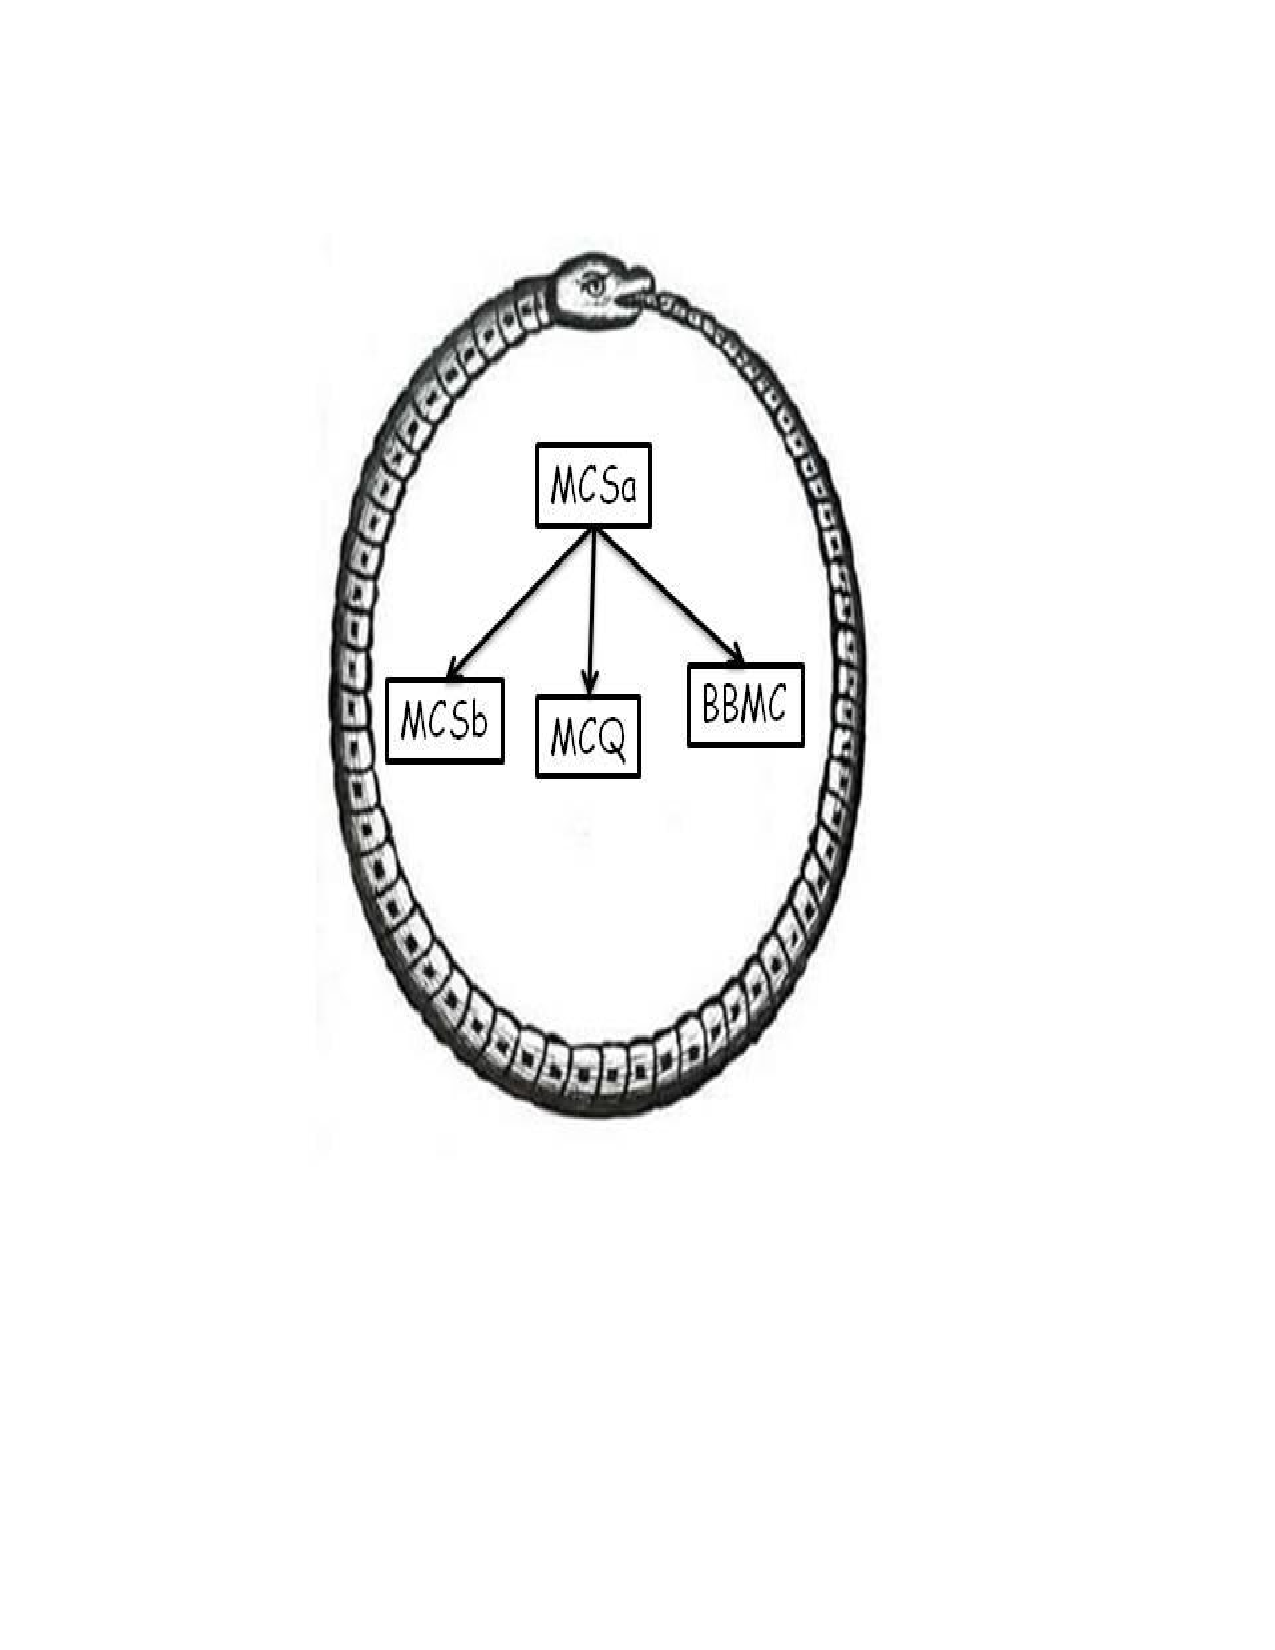
\includegraphics[height=9.2cm,width=13.2cm]{uroboros.pdf}
\vspace{-30mm}
\caption{An alternative hierarchy of the algorithms.}
\label{uroborus}
\end{figure}

The quick brown fox jumped over the lazy dog.
The quick brown fox jumped over the lazy dog.
The quick brown fox jumped over the lazy dog.
The quick brown fox jumped over \cite{ckt} the lazy dog.
The quick brown fox jumped over the lazy dog.
The quick brown fox jumped over the lazy dog.
The quick brown fox jumped over the lazy dog.
The quick brown fox jumped over the lazy dog.

\section{The Lazy Dog}
The quick brown fox jumped over the lazy dog.
The quick brown fox jumped over the lazy dog.
The quick brown fox jumped over the lazy dog.

The quick brown fox jumped over the lazy dog.
The quick brown fox \cite{am97} jumped over the lazy dog.
The quick brown fox jumped over the lazy dog.
The quick brown fox jumped over the lazy dog.
The quick brown fox jumped over the lazy dog.
The quick brown fox jumped over the lazy dog.

%%%%%%%%%%%%%%%%
%              %
%  APPENDICES  %
%              %
%%%%%%%%%%%%%%%%
\begin{appendices}

\chapter{Running the Programs}
An example of running from the command line is as follows:
\begin{verbatim}
      > java MaxClique BBMC1 brock200_1.clq 14400
\end{verbatim}
This will apply $BBMC$ with $style = 1$ to the first brock200 DIMACS instance allowing 14400 seconds of cpu time.

\chapter{Generating Random Graphs}
\label{sec:randomGraph}
We generate Erd\'{o}s-R\"{e}nyi random graphs $G(n,p)$ where $n$ is the number of vertices and
each edge is included in the graph with probability $p$ independent from every other edge. It produces
a random graph in DIMACS format with vertices numbered 1 to $n$ inclusive. It can be run from the command line as follows to produce 
a clq file
\begin{verbatim}
      > java RandomGraph 100 0.9 > 100-90-00.clq
\end{verbatim}
\end{appendices}

%%%%%%%%%%%%%%%%%%%%
%   BIBLIOGRAPHY   %
%%%%%%%%%%%%%%%%%%%%

\bibliographystyle{plain}
\bibliography{bib}

\end{document}
